\documentclass{article}
\usepackage{tikz}
\usepackage{hyperref}
\usetikzlibrary{arrows,shapes}

\begin{document}


\title{Idea Dump : Prompt Engineering DSL}
\author{Fredrik Gustafsson fgn @ github, fredrik.gustafsson@gptmademedoit.com}
\date{\today}

\maketitle

I've been thinking around a DSL for prompt engineering. Here are some of my thoughts. I'm sharing this already is for feedback and something like this might already exists or be in the pipeline. Just injecting small snippets verbatim via placeholders, by add SNIPPET\_PLACEHOLDER into your prompt is pretty straightforward to build, and I've seen many variations of that already. I thinking about generalising that along the lines of composing the injected snippets with other prompts.

\section{Objective}

The objective is to build a tool for creating prompts and managing snippets of knowledge/information, with the ability to inject small snippets of text into the prompts and track the dependencies between different prompts. The key is composition and being able to pull in specific information in a speedy manner when building a prompt. 

\section{Methodology}

Design a domain-specific language (DSL) that allows users to specify prompts and inject snippets of text into them. The DSL should include commands for specifying the prompts, injecting snippets, and applying compositional transformations to the prompts. Use a directed acyclic graph (DAG) to track the dependencies between prompts. Each node in the DAG should represent a prompt, and each edge should represent a dependency between prompts. The metadata associated with each edge should include information about the transformations applied to the prompts, as well as any manual edits that were made.

\section{Example}

\begin{figure}
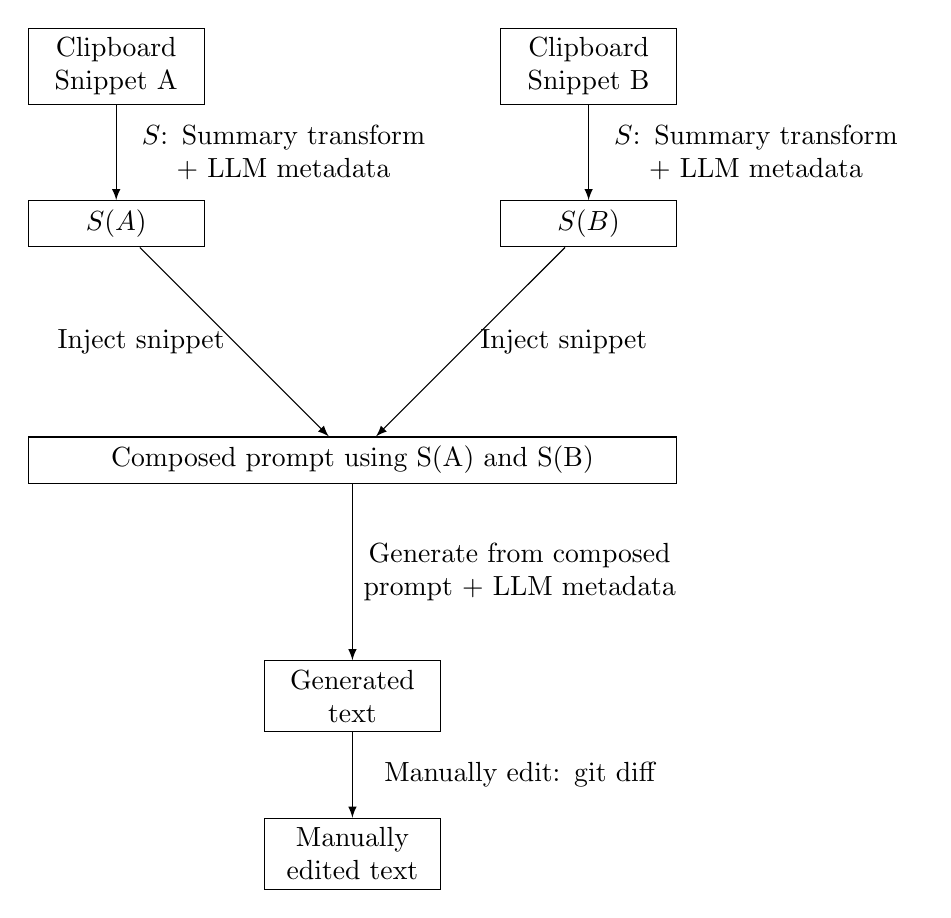
\begin{tikzpicture}[>=latex]
  % Nodes
  \node[rectangle, draw, text width=2cm, align=center] (A) at (0,4) {Clipboard Snippet A};
  \node[rectangle, draw, text width=2cm, align=center] (B) at (6,4) {Clipboard Snippet B};
  \node[rectangle, draw, text width=2cm, align=center] (SA) at (0,2) {$S(A)$};
  \node[rectangle, draw, text width=2cm, align=center] (SB) at (6,2) {$S(B)$};
  \node[rectangle, draw, text width=8cm, align=center] (MPSA) at (3,-1) {Composed prompt using S(A) and S(B)};
  \node[rectangle, draw, text width=2cm, align=center] (C) at (3,-4) {Generated text};
  % made node 'Manually edited text' at (3,-6) {};
  \node[rectangle, draw, text width=2cm, align=center] (D) at (3,-6) {Manually edited text};
  
  % Edges
  \path[->] (A) edge[right, text width=4cm, align=center] node{$S$: Summary transform + LLM metadata} (SA);
  \path[->] (B) edge[right, text width=4cm, align=center] node{$S$: Summary transform + LLM metadata} (SB);
  \path[->] (SA) edge[left] node{Inject snippet} (MPSA);
  \path[->] (SB) edge[right] node{Inject snippet} (MPSA);
  \path[->] (MPSA) edge[right, text width=4cm, align=center] node{Generate from composed prompt + LLM metadata} (C);
 \path[->] (C) edge[right, text width=4cm, align=center] node{Manually edit: git diff} (D);
\end{tikzpicture}
\caption{Graph of the prompt composition dependency graph}
\label{fig:my_label}
\end{figure}

\section{Expected Outcomes}

A tool that allows users to easily create and manage prompts, with the ability to inject snippets of text and track the dependencies between prompts. A detailed record of the prompt DAG, including information about the transformations applied to the prompts and any manual edits that were made. The ability to perform various interesting transformations on the prompt DAG, such as optimizing the prompts or extracting training data from the DAG. Analysis automated chain prompts, like PAL: \href{https://arxiv.org/abs/2211.10435}{Program-aided Language Models}

\section{Data Structure}
The data structure of the Prompt Engineering DSL project can be thought of as a mix of the tree structures in git and the abstract syntax tree commonly generated in compilers. To keep track of the prompts that have been executed and the generated outputs, the tool could use a numbering system similar to the "Out[n]" system used in interactive programming environments such as Jupyter notebooks. In this system, the output of each command is numbered starting with "Out[1]" for the first command, "Out[2]" for the second, and so on. In the context of the Prompt Engineering DSL project, the tool could use this numbering system to label the nodes in the directed acyclic graph (DAG) that represents the prompts. Each node in the DAG would be labeled with the corresponding "Out" number, allowing users to easily refer to specific prompts and their dependencies within the DAG. This numbering system could also be used to label the output generated by the prompts, allowing users to easily refer to specific outputs in future prompts. 

\section{Static and Dynamic Snippets}
Prompts can be injected with both static and dynamic snippets of text. Static snippets are simply chunks of text that are stored and injected into the prompts as is or by piping through transformations. These could be useful for storing frequently used code snippets, notes, or other information that does not change.

Dynamic snippets, on the other hand, are generated by executing programs or making API calls. These snippets are not stored directly, but are instead generated on demand when the prompts are executed. Examples of dynamic snippets include the output of a Python program, the result of a SQL query, or the response from an API call.

\section{Creating and Managing Static Snippets}
Creating static snippets in the Prompt Engineering DSL project should be easy and intuitive. Users should be able to create a new static snippet simply by copying the desired text and storing it in the tool. The tool could provide a modified clipboard manager interface that allows users to easily view, search, and organize their static snippets.

Static snippets can either be explicitly named by the user or automatically named by an language model that looks at the content of the snippet. Explicitly naming static snippets allows users to easily identify and reference specific snippets. 

By providing a simple and efficient way to create and manage static snippets, the Prompt Engineering DSL project will make it easy for users to store and access frequently used information as part of their prompts.

\end{document}